\subsection{Method}
\label{sec:protocol}

We time the communication path with the training loop removed. Timing uses
on-device CUDA events with an explicit synchronisation on the pinned device, and
any diagnostic that transfers a scalar to the host is disabled, because such a
transfer synchronises the device inside the timed region. Implementations are
timed interleaved repetition by repetition rather than in sequential blocks, so
that interference from other tenants lands on all of them at once and their
ratios stay paired; the sequential design produced swings above $100\%$ between
identical configurations on this shared host. The primary statistic is the
minimum over samples, on the modelling assumption that contention adds time
rather than removing it, and the whole timed block is repeated so that the
spread of per-run medians is reported rather than hidden
(Appendix~\ref{app:dispersion}). GPU clocks could not be locked; the account
lacks the privilege. Executed operation counts come from
\texttt{torch.utils.flop\_counter}, so latency is always reported beside the
arithmetic actually performed.

Two decisions about what is compared deserve stating, because both changed our
conclusions. First, we time the attention core --- from queries, keys and values
to the message tensor --- rather than the enclosing module, since the shared
input and output projections are identical across implementations and dilute the
quantity in question. Second, the dense baseline is the better of PyTorch's
fused scaled-dot-product path and a dense attention kernel we wrote ourselves in
Triton, with the same tiling policy and in the same session as the sparse
kernels. At the head widths multi-agent communication uses, the library path is
tuned for a different regime, and comparing a hand-written sparse kernel against
it credits sparsity with the difference between two authors
(Section~\ref{sec:pitfalls}).

Every implementation is checked against the reference at every configuration
whose latency is reported, not at one spot check: exact top-$k$ is discontinuous
in the scores, so two implementations that accumulate the score product in
different orders can rank a near-tied pair differently and then aggregate over
different peers. Maximum deviation across the campaign is at the level of
\texttt{fp32} rounding (Appendix~\ref{app:verification}).

Unless stated otherwise: PyTorch 2.11 with CUDA 12.8 and Triton 3.6,
\texttt{fp32}, head width $d{=}16$, batch $256$, and one NVIDIA Blackwell GPU
shared with other tenants.

\subsection{What the composed implementations cost}
\label{sec:composed}

\begin{table}[t]
\centering\small
\caption{Forward latency (ms, minimum over interleaved samples) of one function
computed six ways, at a quarter of peers retained. The composed sparse path is
slower than every dense implementation at every agent count, and the gap widens
with $N$; the fused sparse kernels change that, and Section~\ref{sec:fused}
reports where.}
\label{tab:headline}
\begin{tabular}{rrrrrrrrrr}
\toprule
& & \multicolumn{4}{c}{\textbf{dense}} & \multicolumn{3}{c}{\textbf{top-$k$}} & \\
\cmidrule(lr){3-6}\cmidrule(lr){7-9}
$N$ & $k$ & unfused & fused & ours & ours & gathered & fused & fused & best sparse \\
& & & (library) & & (tuned) & (composed) & gather & mask & $\div$ best dense \\
\midrule
12 & 2 & 0.012 & 0.013 & 0.004 & 0.004 & 0.022 & 0.004 & 0.006 & 0.99 \\
24 & 4 & 0.015 & 0.011 & 0.004 & 0.004 & 0.028 & 0.006 & 0.016 & 1.37 \\
48 & 8 & 0.020 & 0.015 & 0.008 & 0.008 & 0.048 & 0.012 & 0.024 & 1.54 \\
96 & 16 & 0.045 & 0.033 & 0.018 & 0.014 & 0.120 & 0.049 & 0.039 & 2.80 \\
192 & 32 & 0.136 & 0.072 & 0.036 & 0.034 & 0.424 & 0.387 & 2.305 & 11.29 \\
384 & 64 & 1.082 & 0.220 & 0.119 & 0.108 & 2.405 & 2.750 & 2.025 & 18.70 \\
512 & 128 & 1.899 & 0.349 & 0.188 & 0.172 & 6.435 & 7.214 & 2.662 & 15.44 \\
\bottomrule
\end{tabular}%

\end{table}

The composed sparse path behaves as the manuscript's earlier version reported.
Gathering executes less arithmetic than dense attention --- the counter confirms
the reduction Proposition~\ref{prop:ceiling} permits --- and is nonetheless
slower than every dense implementation at every agent count we measure
(Table~\ref{tab:headline}). Correcting the implementation from masked to
gathered helps at small $N$ and stops helping as $N$ grows, because the gather's
traffic grows faster than the masked path's wasted arithmetic.

The mechanism is memory traffic rather than arithmetic. Gathering does not
remove the score matrix; it adds a compacted $(B,N,k,d)$ tensor and the indices
that build it, and then reads both back. Counting bytes gives a criterion that
is easier to check than the intensity argument it replaces: gathering is
byte-neutral only when the gathered operand is no larger than the score row it
avoids reading, that is when $kd \le N$. At $d{=}16$ and $N{=}512$ that bound is
$k \le 32$, and the quarter-of-peers operating point is four times past it. The
criterion also explains the reversal in which gathering loses to masking at
intermediate $N$, which the earlier version of this manuscript could only
attribute to an inference from its byte accounting.

\subsection{What a purpose-built kernel changes}
\label{sec:fused}

The composed path spends most of its time moving intermediates that a fused
kernel need not create. To bound how much of the measured penalty is that
composition rather than the algorithm, we wrote fused kernels that hold the
score row in registers and never write a score matrix, an index tensor or a
gathered value tensor to memory. Two selection strategies are available to such
a kernel and they trade against each other. Selecting by $k$ successive
argmax-and-mask rounds keeps the aggregation genuinely sparse and makes
selection cost proportional to $k$. Selecting by an exact bisection on the
integer key of the score makes selection cost independent of $k$, but expresses
the retained set as a zero weight rather than by compaction, so the aggregation
performs dense arithmetic however small $k$ is. Both compute the same function
as the composed path.

\begin{figure}[t]
\centering
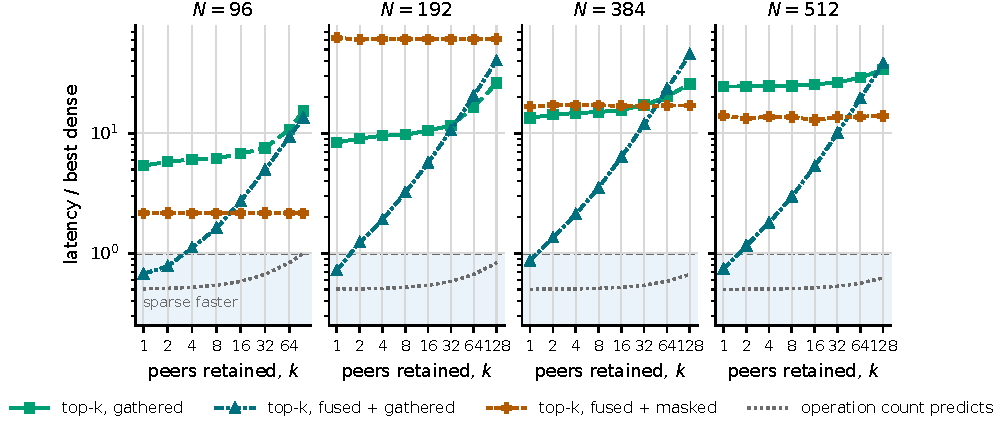
\includegraphics[width=\linewidth]{figures/fig2_ksweep.pdf}
\caption{Latency divided by the faster of the two dense implementations, against
the number of peers retained. The dotted line is what an operation count
predicts for the gathered path, $(N+k)/2N$, which lies below parity everywhere
and so predicts a saving at every sparsity. Shading marks the region in which
sparsity is actually faster; only the fused gathered kernel enters it, and only
at the smallest $k$.}
\label{fig:ksweep}
\end{figure}

\begin{table}[t]
\centering\small
\caption{The sparsity at which a purpose-built sparse kernel stops being faster
than the best dense implementation, and how far it is from parity at the
sparsity multi-agent communication actually uses.}
\label{tab:crossover}
\begin{tabular}{rccrrcrr}
\toprule
& \multicolumn{2}{c}{\textbf{sparsity that pays}} &
  \multicolumn{2}{c}{\textbf{best ratio}} &
  \textbf{replayed, $k{=}1$} &
  \multicolumn{2}{c}{\textbf{at the widest $k$}} \\
\cmidrule(lr){2-3}\cmidrule(lr){4-5}\cmidrule(lr){6-6}\cmidrule(lr){7-8}
$N$ & $k$ & of peers & ratio & at $k$ & min / median & ratio & at $k$ \\
\midrule
192 & $\le 1$ & 0.5\% & 0.76 & 1 & 0.76 / 0.77 & 27.9 & 128 \\
384 & $\le 1$ & 0.3\% & 0.94 & 1 & 0.92 / 0.92 & 18.8 & 128 \\
512 & $\le 1$ & 0.2\% & 0.81 & 1 & 0.77 / 0.77 & 15.4 & 128 \\
\bottomrule
\end{tabular}%

\end{table}

Fusion removes most of the penalty and, at extreme sparsity, reverses the
result. At $512$ agents retaining a single peer, the composed sparse path costs
$4.63$\,ms and the fused one $0.139$\,ms, a factor of $33$ that is attributable
to the implementation and not to the algorithm; the best dense implementation
costs $0.188$\,ms, so the fused sparse path is faster. The manuscript's earlier
claim that no sparse implementation available to us is faster than dense
attention in any measured configuration does not survive, and we report the
correction rather than the claim.

What replaces it is narrower and more useful. A fused sparse kernel is faster
than the best dense implementation only when one or two peers are retained ---
between $0.2\%$ and $2.1\%$ of the available peers, depending on the agent
count --- and the best ratio anywhere in the sweep is $0.66$
(Table~\ref{tab:crossover}). At a quarter of peers, which is the setting the
multi-agent communication literature uses, the best sparse implementation
available to us is $15$ to $26$ times slower than dense attention.

Three things about that crossover matter more than its existence.

The measured advantage stays inside the analytic ceiling. Proposition~\ref{prop:ceiling}
permits at most a twofold reduction in operation count, and the largest speedup
we measure from sparsity, with implementation held constant, is below that. This
is the ceiling behaving as a bound on what is achievable rather than as an
abstraction: once the composed implementation's overheads are removed, the
residual advantage is the one the count allows and no more. It is also why the
first version of these measurements was wrong. Against the library dense path
alone the fused sparse kernel appeared more than twice as fast, which exceeds
what sparsity can supply and was the signal that the baseline, not the
algorithm, was producing the result.

Selection, not aggregation, is what the sparse kernel cannot make cheap. The
argmax-rounds kernel performs $k$ row-wide reductions per query, and reductions
of this shape run at a small fraction of the arithmetic units' throughput
because each is a dependent chain with little instruction-level parallelism.
Its cost is accordingly linear in $k$ and dominates as soon as $k$ exceeds a
handful. The bisection kernel removes that dependence, and the only way it can
is by giving up the compaction --- so the implementation whose selection is cheap
is the one that performs dense aggregation arithmetic. On this hardware a
score-then-select kernel can have sparse arithmetic or $k$-independent
selection, and we could not write one with both.

Fusion is available to dense attention too, and not equally. Dense attention can
stream keys and values in blocks with an online softmax, keeping only a small
tile resident. Exact score-then-select cannot: the complete score row of a query
must exist before the row can be ranked, so the sparse kernel must hold an
$N$-wide tile and its occupancy falls as $N$ grows. That asymmetry is a
consequence of assumption A2 rather than of our implementation, and it is why
the crossover moves to smaller $k$ as the agent count grows.

\subsection{Sensitivity to head width and batch}
\label{sec:sensitivity}

Extending the sweep to head width $512$ resolves a question the earlier version
of this manuscript left open, and resolves it against the direction that version
extrapolated. Reading the ratio down the head-width axis, the crossover exists
only at the two narrowest head widths: the best sparse implementation is faster
than the best dense one at head widths $16$ and $32$ at every agent count, and
at no agent count for head width $128$ or above, where it is roughly twice as
slow (Appendix~\ref{app:grid}). The archival version of this work observed the
ratio falling as head width grew and declined to extrapolate; with the
implementation corrected, the trend runs the other way.

That is what the byte criterion predicts. Byte-neutrality requires
$kd \le N$, so widening the head at fixed agent count tightens the bound on the
retained set proportionally, and at head width $128$ the criterion permits only
$k \le 4$ at $512$ agents --- by which point the selection cost of
Section~\ref{sec:fused} has already overtaken the saving. Widening the batch over a
thirty-twofold range, by contrast, moves the ratio by less than a fifth and
never across parity, which is the expected behaviour of a quantity that is a
ratio of per-element costs.

\subsection{Where the time goes}
\label{sec:stages}

\begin{table}[t]
\centering\small
\caption{Per-stage accounting for both paths at $N{=}\StagesN$. The
last column is the fraction of whichever machine limit binds the stage, and it
separates a stage that is badly implemented from one doing the only thing its
access pattern permits. A figure above $100\%$ marks a stage whose working set
is served from cache, so that its analytic byte count is not traffic to memory;
those stages are the small ones, and none carries an argument.
\StagesCaption}
\label{tab:stages}
\begin{tabular}{lrrrrrrr}
\toprule
\textbf{stage} & GFLOP & GB & FLOP/byte & ms & TFLOP/s & GB/s & \% of limit \\
\midrule
score product & 2.15 & 0.29 & 7.53 & 0.549 & 3.91 & 520 & 35 \\
softmax over $N$ & 0.34 & 0.54 & 0.62 & 0.336 & 1.00 & 1598 & 107 \\
dense aggregation & 2.15 & 0.29 & 7.53 & 0.235 & 9.13 & 1213 & 81 \\
top-$k$ selection & 0.00 & 0.47 & --- & 3.271 & --- & 143 & 10 \\
softmax over $k$ & 0.08 & 0.13 & 0.62 & 0.059 & 1.42 & 2268 & 151 \\
gather of $V$ & 0.00 & 1.21 & --- & 0.954 & --- & 1265 & 84 \\
sparse aggregation & 0.53 & 1.14 & 0.47 & 0.816 & 0.65 & 1398 & 93 \\
\bottomrule
\end{tabular}%

\end{table}

\begin{figure}[t]
\centering
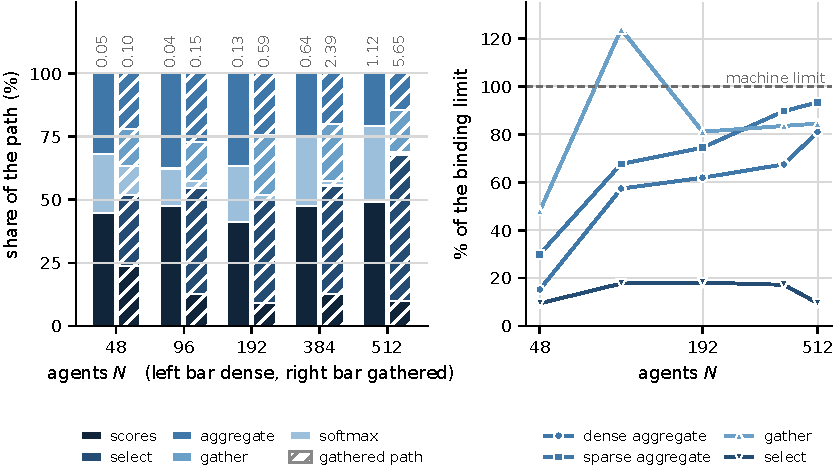
\includegraphics[width=\linewidth]{figures/fig3_stages.pdf}
\caption{\textbf{Left:} how each path divides its time. Selection grows to
dominate the gathered path as the agent count rises. \textbf{Right:} how close
each stage runs to the machine limit that binds it.}
\label{fig:stages}
\end{figure}

Timing each stage in isolation and charging it with its own arithmetic and
traffic corrects an explanation the earlier version of this manuscript offered.
We had attributed the sparse contraction's slowness to a batched
matrix--vector product having lower arithmetic intensity than a real matrix
multiply and being unable to reach the same hardware paths. Measured, that is
wrong. The sparse contraction reaches $93\%$ of the bandwidth the device
attains on a large copy, against $91\%$ for the dense multiply it replaces
(Table~\ref{tab:stages}). Both are bandwidth-saturated and neither is on a
worse hardware path; the sparse one is slower because it moves about four times
the bytes, since the compacted operand carries $kd$ elements per query where the
score row carries $N$. The corrected account is simpler, checkable before the
code is written, and it is the $kd \le N$ criterion of
Section~\ref{sec:composed}.

Selection is a different case, and it is the one stage where the raw
decomposition is misleading in the opposite direction. It is the largest stage
of the composed sparse path, and it runs at under a tenth of the bandwidth the
device attains: it must read the score matrix and write values and indices, and
moving those bytes and nothing else would take a small fraction of the time it
does. That headroom is real, and the fused kernels realise part of it. What no
kernel removes is that the score matrix must be formed and ranked at all, and
the fused measurements of Section~\ref{sec:fused} show what remains once the
headroom is taken.

\subsection{Backward pass and training throughput}
\label{sec:backward}

\begin{table}[t]
\centering\small
\caption{Forward, backward and their sum, for the differentiable
implementations. The sparse path's backward is cheap relative to its forward,
because selection has almost no adjoint, so the gap against fused dense narrows
without closing.}
\label{tab:backward}
\resizebox{\linewidth}{!}{\begin{tabular}{rr rrr rrr rrr rrr r}
\toprule
& & \multicolumn{3}{c}{dense, unfused} & \multicolumn{3}{c}{dense, fused}
& \multicolumn{3}{c}{top-$k$ masked} & \multicolumn{3}{c}{top-$k$ gathered} & \\
\cmidrule(lr){3-5}\cmidrule(lr){6-8}\cmidrule(lr){9-11}\cmidrule(lr){12-14}
$N$ & $k$ & f & b & f+b & f & b & f+b & f & b & f+b & f & b & f+b
& \begin{tabular}[b]{@{}c@{}}gathered f+b\\$\div$ fused f+b\end{tabular} \\
\midrule
192 & 32 & 0.136 & 0.166 & 0.302 & 0.072 & 0.219 & 0.291 & 0.454 & 0.460 & 0.914 & 0.424 & 0.201 & 0.625 & 2.1 \\
384 & 64 & 1.082 & 1.604 & 2.686 & 0.220 & 0.728 & 0.948 & 3.065 & 3.365 & 6.430 & 2.405 & 1.593 & 3.998 & 4.2 \\
512 & 128 & 1.899 & 2.648 & 4.547 & 0.349 & 1.203 & 1.552 & 6.985 & 5.748 & 12.734 & 6.435 & 3.142 & 9.577 & 6.2 \\
\bottomrule
\end{tabular}%
}
\end{table}

Every latency reported so far is a forward pass, which for a training claim is
half the question. Timing forward and backward under the same protocol leaves
the ordering intact and roughly a third of the margin
(Table~\ref{tab:backward}). The gathered path's backward costs about half its
own forward, because the expensive stage --- selection --- has almost no
adjoint: the retained indices are recorded in the forward pass and the backward
is a scatter of gradients into them. Dense attention's backward costs several
times its forward. At $512$ agents the gathered path is $18.5$ times the fused
dense path on the forward alone and $6.3$ times on forward and backward
together; the same narrowing appears at every agent count. The sparse path's
disadvantage in training is therefore substantially smaller than the
forward-only measurements suggest, and remains a disadvantage. The fused kernels are excluded from this comparison: they are
hand-written forward passes, and timing one against an autograd graph would
compare two different things.

\begin{table}[t]
\centering\small
\caption{Where one MAPPO iteration spends its time. Differences between
communication implementations are at or below the iteration-to-iteration spread
in the rightmost column.}
\label{tab:trainstep}
\resizebox{\linewidth}{!}{\begin{tabular}{ll rrrrr rrr}
\toprule
& & \multicolumn{5}{c}{\textbf{share of the iteration (\%)}} & & & \\
\cmidrule(lr){3-7}
$N$ & communication & environment & acting & update fwd & update bwd & optimiser & s/iter & $\div$ fused & spread \\
\midrule
6 & none & 49 & 29 & 11 & 6 & 4 & 2.11 & 1.002 & 4.6 \\
6 & dense, unfused & 48 & 30 & 12 & 6 & 4 & 2.09 & 0.992 & 7.3 \\
6 & dense, library fused & 48 & 30 & 12 & 6 & 4 & 2.10 & 1.000 & 4.0 \\
6 & top-$k$, masked & 48 & 30 & 12 & 6 & 4 & 2.09 & 0.996 & 5.4 \\
6 & top-$k$, gathered & 49 & 29 & 12 & 6 & 4 & 2.13 & 1.011 & 5.3 \\
12 & none & 76 & 14 & 5 & 2 & 2 & 4.35 & 0.998 & 2.3 \\
12 & dense, unfused & 75 & 14 & 6 & 4 & 2 & 4.39 & 1.007 & 3.8 \\
12 & dense, library fused & 75 & 14 & 6 & 3 & 2 & 4.36 & 1.000 & 3.3 \\
12 & top-$k$, masked & 75 & 14 & 6 & 3 & 2 & 4.39 & 1.008 & 5.6 \\
12 & top-$k$, gathered & 75 & 14 & 6 & 4 & 2 & 4.41 & 1.011 & 2.3 \\
24 & none & 92 & 5 & 2 & 1 & 1 & 12.84 & 1.002 & 4.2 \\
24 & dense, unfused & 91 & 5 & 2 & 1 & 1 & 12.98 & 1.013 & 3.3 \\
24 & dense, library fused & 91 & 5 & 2 & 1 & 1 & 12.81 & 1.000 & 1.6 \\
24 & top-$k$, masked & 91 & 5 & 2 & 1 & 1 & 12.80 & 0.999 & 0.8 \\
24 & top-$k$, gathered & 91 & 5 & 2 & 1 & 1 & 12.76 & 0.996 & 1.7 \\
\bottomrule
\end{tabular}%
}
\end{table}

End to end, none of this is visible. Timing a complete training iteration by
phase, with the communication implementation swapped and everything else fixed,
puts the environment at $91\%$ of the iteration at twenty-four agents and
leaves all five implementations within $1.6\%$ of one another, against an
iteration-to-iteration spread of $1.7$ to $3.6\%$ (Table~\ref{tab:trainstep}).
The communication-free variant, which performs no attention at all, is not the
fastest of the five --- which is the clearest available demonstration that this
measurement does not resolve the implementations rather than that it resolves
them as equal. We report it as the null it is. It bounds the practical stakes of
the whole measurement campaign in the regime the training study occupies, and it
is why the computational argument is made on the module in isolation: an effect
a training loop cannot resolve is still an effect, but a paper claiming a
throughput improvement from it would be claiming something it cannot measure.

\subsection{Robustness}
\label{sec:robustness}

The ordering is unchanged under \texttt{torch.compile} and CUDA-graph capture,
at \texttt{bf16}, and on an x86\_64 CPU whose machine balance differs from the
GPU's by more than an order of magnitude. The CPU comparison required
controlling an effect unrelated to attention: with the default allocator the
multi-MiB temporaries each implementation frees between calls are returned to
the kernel and re-faulted on the next call, which at $N{=}192$ adds roughly
$37{,}000$ minor page faults per forward and inflates latency by up to
$8.8\times$. The tax is proportional to the bytes of large temporaries each
implementation churns, so it does not cancel in a ratio, and in an un-pinned run
it inverted the ordering at one configuration. With the heap pinned the
inversion disappears. Appendix~\ref{app:cpu} gives the procedure and both runs.

Because clocks are unlocked and the host is shared, we re-ran the identical
sweep with the device otherwise idle and again under a concurrent load. With the
device idle the ratios reproduce to within a few per cent; under load absolute
latency moves by more than $100\%$ while the paired ratios move by roughly half
that, and every ratio moves against the sparse path. Pairing removes the typical
drift rather than the tail, so the quantity that matters is the margin: no
condition we measured brings a composed sparse implementation below parity, and
the fused crossover reported in Section~\ref{sec:fused} is measured on the
quietest device state we could obtain. Appendix~\ref{app:drift} gives the
figures.
